\section{Evaluation of Solar Cell Models}\label{sec:evaluation_of_solar_cell_models}

To evaluate these solar cell models and their proposed modifications, we used a
set of almost 450 Maxeon Gen III and Maxeon C60 solar cells. In this section, we
will discuss the aspects of this collection, how we characterized the solar
cells to generate a robust dataset with custom \acf{HW} and \acf{SW}, and
techniques (both experimental and statistical) to evaluate and estimate their
parameters. Finally, we'll use these parameters to compare the models and their
real world equivalents to determine model accuracy and precision.


\subsection{Solar Cell Dataset}\label{subsec:solar_cell_dataset}

The solar cells used for the \ac{LHRs} solar vehicle are a mixture of Maxeon Gen
III and Maxeon C60 solar cells. These solar cells were selected primarily due to
financial and availability constraints; historically, in the last two solar
vehicle revisions (2018, 2021) Gen III Bin Le1 cells have been used, but this
year the team decided to procure cheaper, more easily available C60 cells from
secondary suppliers. Regardless, both of these cell lines remain state of the
art despite their age \footnote{dates are unclear, but it appears that C60 was
introduced around 2007\cite{sunpower_history} and the Gen III has been around as
long as 2013\cite{smith_et_al}.}; both Aptera Motors\cite{aptera_solar_cells}
and Lightyear One\cite{lightyear_one_solar_cells} -the latter of which is a
former Solar Vehicles team- have announced cooperation with Maxeon to use their
solar cells. Aptera in particular uses the Gen III
cells\cite{aptera_solar_cells}.

While these cell types are both $125 \si{\mm}$ by $125 \si{mm}$ (see
\autoref{fig:maxeon_gen_iii_cell_footprint} for a visualization of the cell
physical layout), the Gen III cells are slightly more efficient than the C60
cells. Their (Gen III) rear contacts also tend to be slightly narrower than the
C60 cells. Their electrical characteristics are outlined in
\autoref{fig:maxeon_gen_iii_cell_characteristics} and
\autoref{fig:maxeon_c60_cell_characteristics}. Note that the Maxeon Gen III
cells are explicitly Bin Le1 cells, although the dataset will later show that
the binning for both groups of cells tends to not be very respective of the
actual measured \ac{I-V} curves, which is likely due to the variance in our
testing setup.

Since these cells were unpacked and designated for specific years,
\autoref{table:solar_cell_dataset} is provided to delineate between the
different types and `lines' of cells tested. `Lines' in this sense indicate
the academic year the cells were originally unpacked and tested.

\begin{figure}[!htbp]
    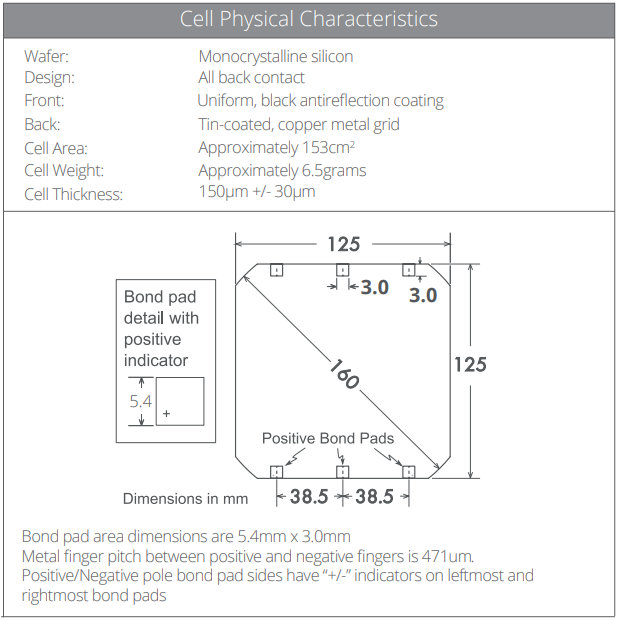
\includegraphics[width=\textwidth]{maxeon_gen_iii_cell_footprint.png}
    \caption{Maxeon Gen III Cell Footprint}
    \label{fig:maxeon_gen_iii_cell_footprint}
\end{figure}

\begin{figure}[!htbp]
    \centering
    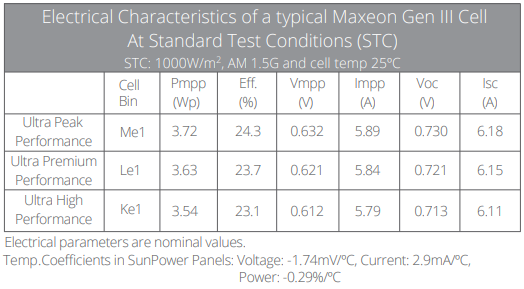
\includegraphics[width=0.8\textwidth]{maxeon_gen_iii_cell_characteristics.png}
    \caption{Maxeon Gen III Cell Characteristics}
    \label{fig:maxeon_gen_iii_cell_characteristics}
\end{figure}

\begin{figure}[!htbp]
    \centering
    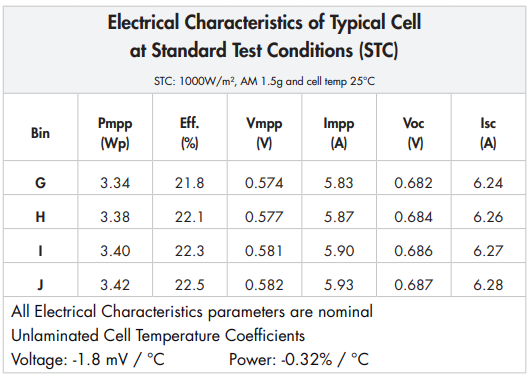
\includegraphics[width=0.8\textwidth]{maxeon_c60_cell_characteristics.png}
    \caption{Maxeon C60 Cell Characteristics}
    \label{fig:maxeon_c60_cell_characteristics}
\end{figure}

\begin{table}[!htbp]
    \begin{tabularx}{\textwidth}{
        | >{\raggedright\arraybackslash}X
        | >{\raggedright\arraybackslash}X
        | >{\raggedright\arraybackslash}X
        | >{\raggedright\arraybackslash}X | }
        \hline
        Cell Line   & Year Unpacked & Type      & Number of Cells \\ \hline \hline
        RP          & 2022          & C60       & X               \\ \hline
        MW          & 2020          & Gen III   & X               \\ \hline
        2019\_Le1   & 2019          & Gen III   & X               \\ \hline
        BU          & 2018          & Gen III   & X               \\ \hline
    \end{tabularx}
    \caption{Cell Lines Used in Solar Cell Dataset}
    \label{table:solar_cell_dataset}
\end{table}
\todo[inline]{Add number of cells tested to each group in table.}


\subsection{Characterizing Solar Cells}\label{subsec:characterizing_solar_cells}

\todo[inline,caption={}]{
    \begin{itemize}
        \item Introduction to proposed testing setup (add image)
        \item Discussion of light source,
        https://www.mpja.com/download/34769opdata.pdf MPJA grow lights, spectrum
        \item Discussion of irradiance control, Blackbody C (refer to Appendix C)
        \item Discussion of how to measure the solar cell (refer to Appendix D)
        \item Process of characterizing solar cell (assembly, test, disassembly)
    \end{itemize}
}

To characterize solar cells, we develop a test setup as outlined in
\autoref{fig:cell_test_setup}. In this test setup, we maintain three critical
requirements:

\begin{itemize}
    \item The test article shall receive a \textit{measurable} and
    \textit{consistent} irradiance over the test duration.
    \item The test article shall receive a \textit{uniform} irradiance over the
    span of the test article.
    \item The test article shall maintain a \textit{measurable} and
    \textit{consistent} surface temperature over the test duration.
\end{itemize}

To achieve these aforementioned requirements, a solar cell or solar module of up
to $500 \si{\mm}$ by $250 \si{mm}$ (equivalent to 4 cells by 2 cells) in size is
placed upon a thermal bed separated by a thin, electrically insulating layer of
Kapton tape; the photovoltaic is maintained at a fixed temperature by the
thermal bed through conduction, which is controlled by a \todo{Insert name of
heater/ chiller device} XXX. A solar simulator, consisting of a set of dimmable
grow light modules (MPJA 34769-OPs), is mounted to an aluminum plate heatsink.
Because these light modules have an nonuniform intensity profile (e.g. light is
concentrated radially from the center of the fixture), they are spaced relative
to each other such that overlapping regions of lights at a fixed distance from
the surface of the photovoltaic return a roughly uniform light distribution. The
spacing is empirically evaluated using a light intensity sensor (TSL2591),
similar to how \acf{PPFD} is measured\cite{ppfd_measurement}; a closely spaced
set of points is evaluated and the intensity measurements are plotted to
determine the variance in intensity. \autoref{fig:light_spacing_coherence}
demonstrates (a) the ratio of the light source to the solar cell, (b) how the
distance between the two centers of nearby light sources can be cohered, and (c)
how the distance from the light source and the solar cell affects the area that
can be cohered. It is generally accepted that as the light source moves away
from the cell, the intensity of light drops off by the cube of the distance and
nearby lights need to be spaced farther apart to maintain uniformity.

\begin{figure}[!htbp]
    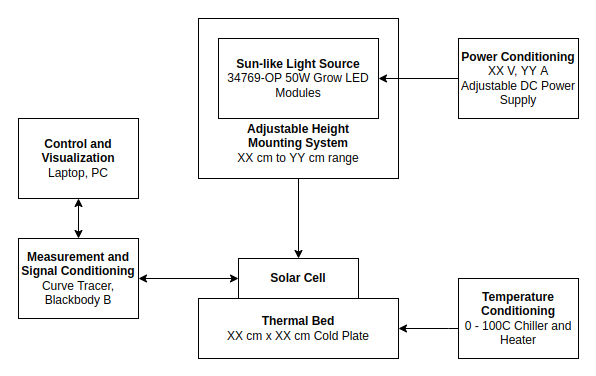
\includegraphics[width=\textwidth]{cell_test_setup.png}
    \caption{Photovoltaic Testing Setup}
    \label{fig:cell_test_setup}
\end{figure}

\begin{figure}[h]
    \centering
    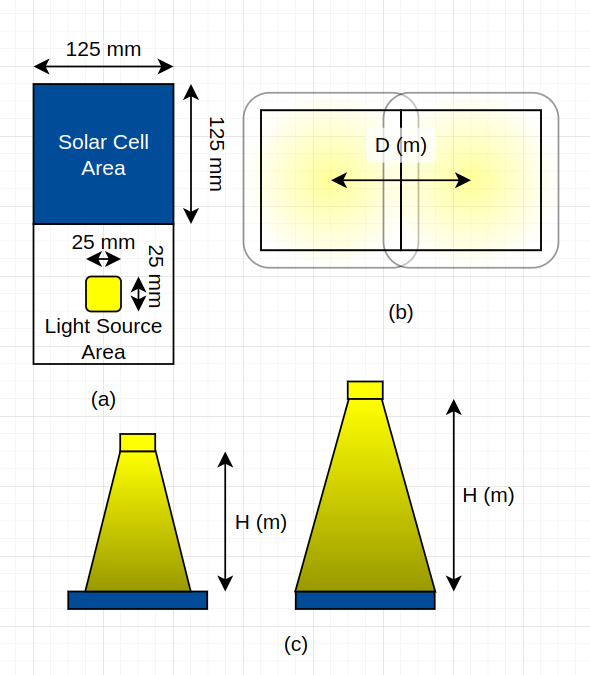
\includegraphics[width=0.6\textwidth]{light_spacing_coherence.png}
    \caption{Grow Light Spacing and Coherence}
    \label{fig:light_spacing_coherence}
\end{figure}

To achieve the last unmet requirement, \textit{the test article shall receive a
measurable and consistent irradiance over the test duration}, the same light
sensor is used to measure the intensity of light over a fixed period of time.
This period of time should be long enough to determine whether the lights have a
warm up time and change in irradiance over the expected experiment duration.
The TSL2591 returns values in counts according to its datasheet, which can be
converted into $\si{watt}/\si{\meter}^2$. However, the normalized responsivity
spectrum of the TSL2591 (\autoref{fig:tsl2591_spectral_responsivity}) is quite
divergent from AM1.5G solar spectrum; this means that the real irradiance will
be off significantly. In order to calibrate the readings from the sensor as a
proxy for the real irradiance experienced by the solar cell, we need to compare
it to either a known source or a reference pyrometer. Another way to interpret
the readings in counts is to convert it into lux; Michael et
al.\cite{michael_et_al} proposes several methodologies for determining and
verifying a $\si{\lux}$ to $\si{\watt}/\si{\meter}^2$ conversion factor. They
also propose an `engineering rule of thumb', that $120 \si{\lux} =
\si{\watt}/\si{\meter}^2$.
\todo[inline]{Add potential note later on about needing teflon to filter in
saturation conditions - can this fixed by adjusting gain/integration time?}
\todo[inline]{Reference Gacusan's, Burgt's thesis regarding designing low-cost
pyranometer using TSL2591 and TSL2591-like sensors}

\begin{figure}[!htbp]
    \centering
    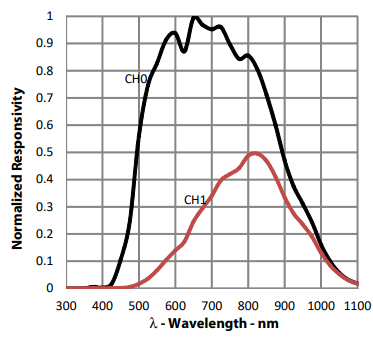
\includegraphics[width=0.5\textwidth]{tsl2591_spectral_responsivity.png}
    \caption{TSL2591 Spectral Responsivity}
    \label{fig:tsl2591_spectral_responsivity}
\end{figure}
\todo[inline]{Add referenceto AMS TSL2591 datasheet. Figure 11.}


\subsection{Experimental Extraction of Cell Parameters}\label{subsec:experimental_extraction_of_cell_parameters}

\todo[inline,caption={}]{
    \begin{itemize}
        \item Present results of each cell line
        \item Compare against smith et al for Gen III how accurate and precise
        the cell distribution is
        \item Review parameters that need to be measured empirically (\ac{RS}, \ac{RSH}, etc)
        \item Discussion on how to measure series and shunt resistance
        empirically (refer to Appendix E)
        \item Discussion on how to measure temperature coefficients empirically
    \end{itemize}
}


\subsection{Statistical Extraction of Cell Parameters}\label{subsec:statistical_extraction_of_cell_parameters}

\todo[inline,caption={}]{
    \begin{itemize}
        \item Review parameters that could be estimated statistically (\ac{alpha}, \ac{beta}, etc)
        \item Discussion on curve fitting techniques
    \end{itemize}
}


\subsection{Modeling Solar Cell Datasets}\label{subsec:modeling_solar_cell_datasets}

\todo[inline,caption={}]{
    \begin{itemize}
        \item Discuss python model for modeling cells, iterative solving (refer
        to Appendix F)
        \item Present initial figures showing expected model output
    \end{itemize}
}


\subsection{Evaluating Solar Cell Models}\label{subsec:evaluating_solar_cell_models}
